\documentclass[notitlepage]{article}
\usepackage[utf8]{inputenc} 
\usepackage{geometry} 		
\usepackage{chngcntr}
\usepackage{amsmath} 			
\usepackage{amssymb}			
\usepackage{mathtools}		
\usepackage{comment} 			
\usepackage{mdframed}			
\usepackage{xcolor}				
\usepackage{fancyhdr}			
\usepackage{listings}			
\usepackage{color}				
\usepackage{tikz}	
\usepackage{tasks}			
\usepackage{exsheets}		
\usepackage{array}			
\usepackage{empheq}
\usepackage{caption}
\usepackage{pdfpages}
\usepackage{tabularx}

\geometry{ 						%Format titlepage (interrupted by newgeometry)
	a4paper,
	total={170mm,257mm}%,
	%left=0mm,
	%top=0mm,
}

%START DEFINE YOUR VARIABLES HERE

\newcommand{\documentName}{User Manual}
\newcommand{\projectName}{Label Refinement by Behavioral Similarity - WEBSITENAME}

%END DEFINE YOUR VARIABLES HERE

\title{%
	\documentName\text{ } \\
  \large \projectName\text{ } \\
  }

\author{
	\large \underline{Document owners:}\\ 
	Bianka Bakullari\\
	\texttt{}
	Christopher Beine\\
	\texttt{}
	Nicole Ventsch\\
	\texttt{}
	Juan Garza\\
	\texttt{}
}

\date{\small{Last edited: \today}}

\pagestyle{fancy}
\fancyhf{}
\rhead{}
\lhead{\documentName\space-\space\projectName}

\makeatletter					%Prefix to add ToC to titlepage
\newcommand*{\toccontents}{\@starttoc{toc}}
\renewcommand*\contentsname{}
\makeatother
                  

\begin{document}

\begin{titlepage}
\clearpage\maketitle			%Clear title page
\thispagestyle{fancy}
\tableofcontents
\end{titlepage}

\rfoot{\thepage}				%Start printing page-numbers, after title page.

\newgeometry{ 					%Default page formatting on-going #1
	total={170mm,257mm},
	left=20mm,
	top=25mm,
    bottom=30mm					%Causes warning
}

\begin{flushleft}				%Default page formatting on-going #2

\section{Overview}

Many processes involve carrying out an action multiple times. An example for this would be an online shop in which you first have to pay a registration fee before ordering an item and paying it. This process contains the event ``payment" twice, but in different contexts, so that the payments are actually two different tasks. In the context of analysing processes, the event logs usually only contain the event names, so that the ``payment" actions would be treated as the same task and loops would be induced in the resulting models. However, these loops do not match the actual process, which is the issue this project addresses. 

Using the webservice we provide, imprecise logs can be refined based on the structural contexts of the events. The refinement is executed by relabeling the original log and no filtering is applied to the log. Moreover, it is possible for the user to interactively change the thresholds used by the algorithm. The algorithm we use is based on \cite{paper}.

In the following chapters, the usage of this web service will be explained.




\section{The Start Page}

The start page of our web service consists of different parts, which will be explained in the following subsections. Namely, we have the parts "Upload Event Log for refining" (1), "Customize" (2), "Last uploaded files" (3) and "Last refined files" (4), which can be viewed in Figure 1.

\begin{figure}[h]
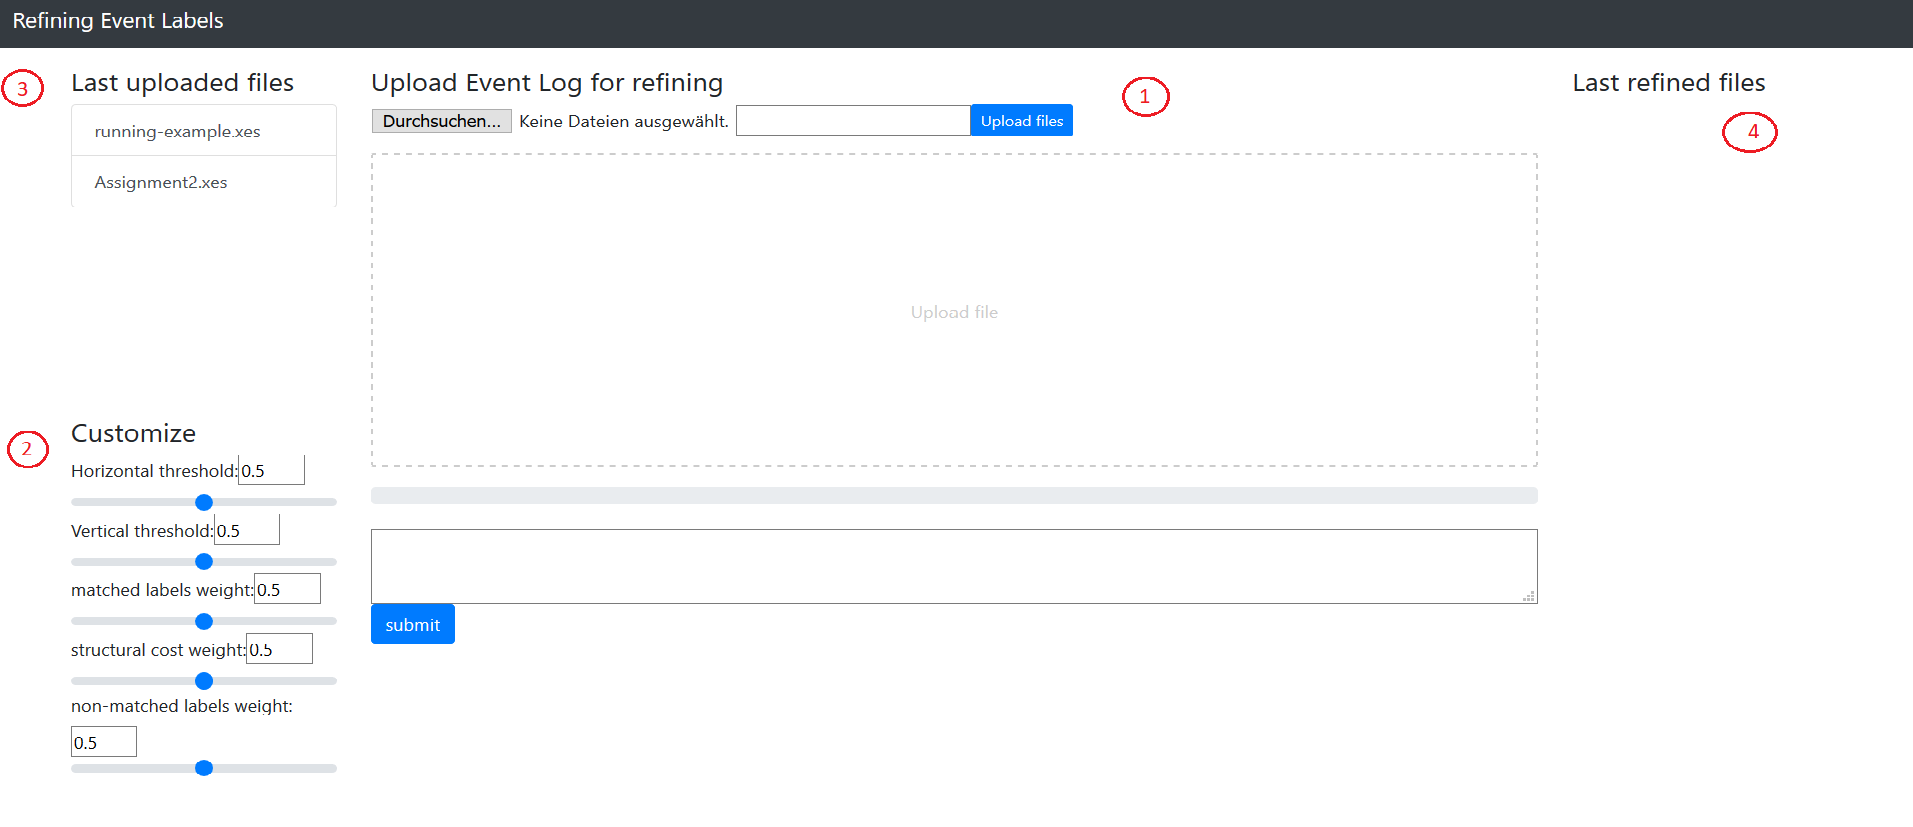
\includegraphics[scale=0.42]{startpage.png}
\caption{Overview of the start page with the different parts marked in red numbers}
\end{figure}

\subsection{Upload Event Log for refining}
In this part of the start page, an event log can be uploaded. In order to do so, the user can either directly type in a path to a file and press the "Upload files" button or he can use the "search" button to search local files on your pc or drag a file into the big box with "upload file" written in it. Afterwards, he has to press the "Upload files" button in order to upload the selected file, he can add a comment on the file in the blanc box and press submit to start the upload. 

In order to successfully upload a file, this file has to be in XES or csv format, otherwise an error will occur. 

\subsection{Customize}
In this section, the user can adjust the thresholds in order to fit his needs. To do so, he can either adjust them using the provided slide control or by typing them manually. The thresholds the user can adjust are the horizontal threshold, the vertical threshold, the weight structure, the weight for matched pairs of actions and the weight for not matched pairs of actions.

\subsection{Last uploaded files}
In this part of the start page, the user can see up to five of his last uploaded files. These files are not refined yet.

\subsection{Last refined files}
In this part of the start page, the user can see up to five of his last refined files. These files are already refined.



%\addcontentsline{toc}{chapter}{\textbf{References}}
\end{flushleft}
%\bibliography{uw-ethesis}
% Tip 5: You can create multiple .bib files to organize your references. 
% Just list them all in the \bibliogaphy command, separated by commas (no spaces).

% The following statement causes the specified references to be added to the bibliography% even if they were not 
% cited in the text. The asterisk is a wildcard that causes all entries in the bibliographic database to be included (optional).


\begin{thebibliography}{5}
\bibitem{paper}
Lu, Xixi, et al. "Handling duplicated tasks in process discovery by refining event labels." International Conference on Business Process Management. Springer, Cham, 2016.

\bibitem{}
La Rosa M., Loos P., Pastor O. (eds) Business Process Management, BPM 2016, Lecture Notes in Computer Science, vol 9850. Springer, Cham, 2016.






\end{thebibliography}










\end{document}
